\begin{figure}[!t]
    \centering
    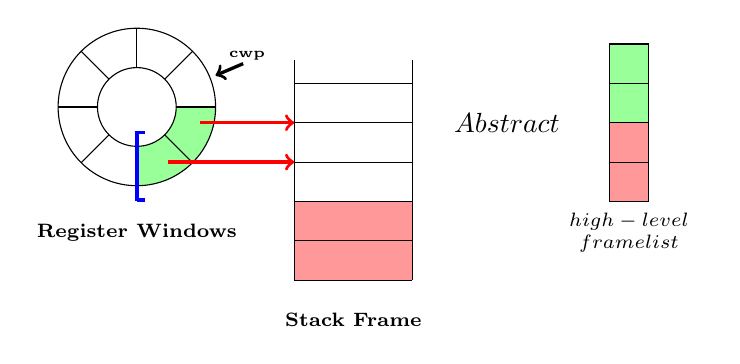
\begin{tikzpicture}
        \fill[green!40!white] (0,0) -- (0,-1cm) arc (-90:0:1cm) -- (0,0);
        \draw (0, 0) -- (90:1cm);
        \draw (0, 0) -- (45:1cm);
        \draw (0, 0) -- (0:1cm);
        \draw (0, 0) -- (-45:1cm);
        \draw (0, 0) -- (-90:1cm);
        \draw (0, 0) -- (-135:1cm);
        \draw (0, 0) -- (-180:1cm);
        \draw (0, 0) -- (135:1cm);
        \fill[white] (0, 0) circle (0.5cm);
        \draw (0, 0) circle (1cm);
        \draw (0, 0) circle (0.5cm);
        \draw[very thick, blue] (0, -0.3) -- (0, -1.2);
        \draw[very thick, blue] (0, -0.32) -- (0.1, -0.32);
        \draw[very thick, blue] (0, -1.18) -- (0.1, -1.18);

        \node(cwp) at (1.4, 0.65) {\tiny \bf cwp};
        \draw[->, very thick] (1.35, 0.55) -- (1, 0.4);

        \node(regwin) at (0, -1.6) {\scriptsize \bf Register Windows};

        %%%%%%%%%%%%%%%%%%%%%%%%%%%%%%%%%%%%%%%%%%%%%%%%%%%%%%

        \fill[red!40!white] (2, -1.2) rectangle (3.5, -1.7);
        \fill[red!40!white] (2, -1.7) rectangle (3.5, -2.2);

        \draw[-] (2, 0.6) -- (2, -2.2);
        \draw[-] (3.5, 0.6) -- (3.5, -2.2);
        
        \draw[-] (2, 0.3) -- (3.5, 0.3);
        \draw[-] (2, -0.2) -- (3.5, -0.2);
        \draw[-] (2, -0.7) -- (3.5, -0.7);
        \draw[-] (2, -1.2) -- (3.5, -1.2);
        \draw[-] (2, -1.7) -- (3.5, -1.7);
        \draw[-] (2, -2.2) -- (3.5, -2.2);

        \node(stkfm) at (2.75, -2.7) {\scriptsize \bf Stack Frame};

        %%%%%%%%%%%%%%%%%%%%%%%%%%%%%%%%%%%%%%%%%%%%%%%%%%%%%%%

        \draw[->, very thick, red] (0.8, -0.2) -- (2, -0.2);
        \draw[->, very thick, red] (0.4, -0.7) -- (2, -0.7);

        %%%%%%%%%%%%%%%%%%%%%%%%%%%%%%%%%%%%%%%%%%%%%%%%%%%%%%

        \node(abstract) at (4.7, -0.2) {$\xLongrightarrow{\text{Abstract}}$};

        %%%%%%%%%%%%%%%%%%%%%%%%%%%%%%%%%%%%%%%%%%%%%%%%%%%%%%

        \fill[green!40!white] (6, 0.8) rectangle (6.5, 0.3);
        \fill[green!40!white] (6, 0.3) rectangle (6.5, -0.2);
        \fill[red!40!white] (6, -0.2) rectangle (6.5, -0.7);
        \fill[red!40!white] (6, -0.7) rectangle (6.5, -1.2);

        \draw[-] (6, 0.8) -- (6, -1.2);
        \draw[-] (6.5, 0.8) -- (6.5, -1.2);

        \draw[-] (6, 0.8) -- (6.5, 0.8);
        \draw[-] (6, 0.3) -- (6.5, 0.3);
        \draw[-] (6, -0.2) -- (6.5, -0.2);
        \draw[-] (6, -0.7) -- (6.5, -0.7);
        \draw[-] (6, -1.2) -- (6.5, -1.2);

        \node(hfrmlist) at (6.25, -1.6) 
            {
                \scriptsize \bf
                $
                \begin{array}{c}
                    \text{high-level} \\
                    \text{framelist}
                \end{array}
                $
            };
    \end{tikzpicture} 
    \caption{Abstraction of Register Windows and Memory}
    \label{fig:Abstraction of Register Windows and Memory}
    \vspace{-0.5em}
\end{figure}